\chapter{Johdanto}

\section{Laskennalliset ongelmat}

Tämän kurssin tarkoituksena on opettaa menetelmiä,
joiden avulla voimme ratkaista \emph{tehokkaasti}
laskennallisia ongelmia.
Lähtökohtana on, että meille annetaan ongelman kuvaus,
jossa kerrotaan täsmällisesti algoritmille annettava
syöte sekä haluttu tuloste.
Syöte tarkoittaa, mitä tietoja algoritmille annetaan,
ja tuloste tarkoittaa, mitä algoritmin tulee tuottaa vastauksena.

Seuraavassa on esimerkki laskennallisesta ongelmasta:

\begin{itemize}
\item \textbf{Syöte}: Algoritmille annetaan taulukko,
jossa on $n$ kokonaislukua, sekä kokonaisluku $x$.
\item \textbf{Tuloste:} Algoritmin tulee ilmoittaa,
monellako tavalla voimme valita taulukosta kaksi eri
kohdissa olevaa lukua, joiden summa on $x$.
\end{itemize}

Ohjelmoinnin peruskursseilla olemme oppineet taitoja,
joiden avulla voimme ratkaista laskennallisia ongelmia.
Esimerkiksi yllä olevan ongelman voisi ratkaista seuraavalla algoritmilla,
joka olettaa, että luvut ovat taulukossa \texttt{taulu},
ja laskee tapojen määrän muuttujaan \texttt{tulos}.

\begin{code}
int tulos = 0;
for (int i = 0; i < n; i++) {
    for (int j = i+1; j < n; j++) {
        if (taulu[i]+taulu[j] == x) {
            tulos++;
        }
    }
}
\end{code}

Ensimmäinen vaihe algoritmiikan oppimisessa on oppia
ohjelmoinnin perustaidot niin, että osaamme kirjoittaa
jonkin toimivan koodin, joka ratkaisee annetun ongelman.
Toinen vaihe, johon keskitymme tällä kurssilla,
on oppia suunnittelemaan \emph{tehokkaita} algoritmeja.
Tämä tarkoittaa, että haluamme saada mahdollisuuksien mukaan
aikaan jotain parempaa kuin suoraviivaisia
raakaan voimaan perustuvia algoritmeja.

Algoritmien tehokkuudella on suuri merkitys käytännössä.
Esimerkiksi Google-haku on käyttökelpoinen sen vuoksi,
että saamme hakutulokset heti haun lähettämisen jälkeen.
Jos meidän tulisi odottaa tuloksia vaikkapa viikko,
tämä rajoittaisi paljon haun käyttömahdollisuuksia.
Toinen esimerkki on reittihaku, joka kertoo meille parhaan
tavan matkustaa lähtöpaikasta kohdepaikkaan.
Tässäkin palvelussa olennainen osa käyttökokemusta on,
että saamme reitin välittömästi haun jälkeen eikä meidän tarvitse odottaa.

Kiehtova piirre algoritmiikassa on, että monimutkaisetkin algoritmit
syntyvät yksinkertaisista aineksista. Keskeiset käsitteet ovat

\begin{itemize}
\item muuttujat, joissa voimme säilyttää tietoa ohjelmassa,
\item ehtolause (\texttt{if}), jonka avulla voimme haarautua ohjelmassa,
\item silmukat (\texttt{for} ja \texttt{while}), joiden avulla voimme
toistaa laskentaa, sekä
\item taulukot, joissa voimme säilyttää suurta määrää tietoa.
\end{itemize}

Itse asiassa voimme toteuttaa minkä tahansa algoritmin vain näitä
aineksia käyttäen.
Tämä on huojentava tieto, koska meidän ei siis tarvitse opetella
suurta määrää ohjelmointikielten ominaisuuksia,
ennen kuin voimme alkaa suunnitella algoritmeja.
Vaikeutena on kuitenkin \emph{keksiä}, kuinka käyttää näitä
tekniikoita eri tilanteessa.

\section{Rekursiiviset algoritmit}

Rekursio on kätevä työkalu, jonka avulla voimme käydä
järjestelmällisesti läpi kaikki tavat ongelman ratkaisuun.
Seuraavaksi tutustumme esimerkkeihin rekursion käyttämisestä.

\subsection{Osajoukkojen läpikäynti}

Joukon osajoukkoja ovat kaikki tavat valita osa joukon alkioista.
Esimerkiksi joukon $\{1,2,3\}$ osajoukot ovat
$\emptyset$ (tyhjä joukko), $\{1\}$, $\{2\}$, $\{3\}$,
$\{1,2\}$, $\{1,3\}$, $\{2,3\}$ ja $\{1,2,3\}$.
Jos joukossa on $n$ alkioita, osajoukkoja on $2^n$.

Rekursio tarjoaa kätevän tavan käydä läpi kaikki
joukon osajoukot. Esimerkiksi seuraava koodi pitää yllä
rakennetta

\begin{code}
ArrayDeque<Integer> osajoukko;
\end{code}

joka sisältää vuorollaan kunkin joukon $\{1,2,\dots,n\}$
osajoukon. Rekursiivista metodia \texttt{muodosta} kutsutaan
parametrilla $1$.

\begin{code}
void muodosta(int x) {
    if (x == n+1) {
        System.out.println(osajoukko);
        return;
    }
    muodosta(x+1); // x ei valita osajoukkoon
    osajoukko.addLast(x);
    muodosta(x+1); // x valitaan osajoukkoon
    osajoukko.removeLast(x);
}
\end{code}

Jokaisessa kutsussa metodi käy läpi tapaukset,
otetaanko luku $x$ mukaan osajoukkoon vai ei.
Molemmissa tapauksissa metodi kutsuu itseään yhtä
suuremalla $x$:n arvolla.
Lopulta kun $x=n+1$, kaikki luvut on käyty läpi
ja on aika tulostaa osajoukko.

Esimerkiksi tapauksessa $n=3$ koodin tulostus on seuraava:

\begin{code}
[]
[3]
[2]
[2, 3]
[1]
[1, 3]
[1, 2]
[1, 2, 3]
\end{code}

\subsection{Permutaatioiden läpikäynti}

Joukon permutaatiot ovat kaikki tavat järjestää joukon alkiot.
Esimerkiksi joukon $\{1,2,3\}$ permutaatiot ovat
$(1,2,3)$, $(1,3,2)$, $(2,1,3)$, $(2,3,1)$, $(3,1,2)$ ja $(3,2,1)$.
Jos joukossa on $n$ alkiota, permutaatioita on $n!$.

Myös permutaatioiden läpikäynti onnistuu kätevästi rekursiolla.
Seuraava koodi pitää yllä rakennetta

\begin{code}
ArrayDeque<Integer> permutaatio;
\end{code}

joka sisältää vuorollaan kunkin joukon $\{1,2,\dots,n\}$ permutaation.
Rekursiivista metodia \texttt{muodosta} kutsutaan ilman parametreja.

\begin{code}
void muodosta() {
    if (permutaatio.size() == n) {
        System.out.println(permutaatio);
        return;
    }
    for (int i = 1; i <= n; i++) {
        if (!permutaatio.contains(i)) {
            permutaatio.addLast(i);
            muodosta();
            permutaatio.removeLast();
        }
    }
}
\end{code}

Tässä on ideana, että metodi käy joka kutsulla läpi kaikki luvut
$1,2,\dots,n$ ja aina jos luku ei kuulu vielä permutaatioon,
koodi haarautuu rekursiivisesti tapaukseen, jossa se lisätään
seuraavaksi permutaatioon.
Sitten kun permutaatiossa on $n$ lukua, se on valmis ja
voimme tulostaa sen.

Esimerkiksi tapauksessa $n=3$ koodin tulostus on seuraava:

\begin{code}
[1, 2, 3]
[1, 3, 2]
[2, 1, 3]
[2, 3, 1]
[3, 1, 2]
[3, 2, 1]
\end{code}

\subsection{Peruuttava haku}

Peruuttava haku on yleinen rekursiivinen menetelmä,
joka muodostaa järjes\-telmällisesti kaikki ratkaisut tehtävään.
Siinä on ideana aloittaa tyhjästä ratkaisusta ja käydä
joka askeleella läpi kaikki mahdolliset tavat laajentaa ratkaisua.

\begin{figure}
\center
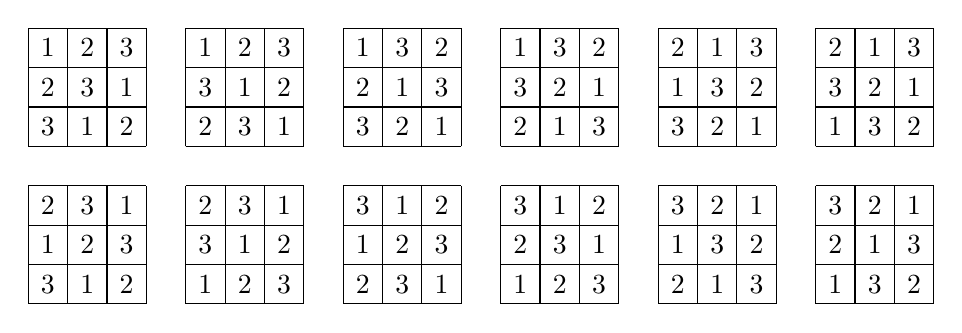
\begin{tikzpicture}[scale=0.5]
\newcommand\nelio[9]{
\draw (0,0) grid (3,3);
\foreach \x/\y/\v in {0/0/#1,1/0/#2,2/0/#3,0/1/#4,1/1/#5,2/1/#6,0/2/#7,1/2/#8,2/2/#9} \node at (0.5+\x,2.5-\y) {\v};
}
\begin{scope}
\nelio{1}{2}{3}{2}{3}{1}{3}{1}{2}
\end{scope}
\begin{scope}[xshift=4cm]
\nelio{1}{2}{3}{3}{1}{2}{2}{3}{1}
\end{scope}
\begin{scope}[xshift=8cm]
\nelio{1}{3}{2}{2}{1}{3}{3}{2}{1}
\end{scope}
\begin{scope}[xshift=12cm]
\nelio{1}{3}{2}{3}{2}{1}{2}{1}{3}
\end{scope}
\begin{scope}[xshift=16cm]
\nelio{2}{1}{3}{1}{3}{2}{3}{2}{1}
\end{scope}
\begin{scope}[xshift=20cm]
\nelio{2}{1}{3}{3}{2}{1}{1}{3}{2}
\end{scope}
\begin{scope}[yshift=-4cm]
\nelio{2}{3}{1}{1}{2}{3}{3}{1}{2}
\end{scope}
\begin{scope}[yshift=-4cm,xshift=4cm]
\nelio{2}{3}{1}{3}{1}{2}{1}{2}{3}
\end{scope}
\begin{scope}[yshift=-4cm,xshift=8cm]
\nelio{3}{1}{2}{1}{2}{3}{2}{3}{1}
\end{scope}
\begin{scope}[yshift=-4cm,xshift=12cm]
\nelio{3}{1}{2}{2}{3}{1}{1}{2}{3}
\end{scope}
\begin{scope}[yshift=-4cm,xshift=16cm]
\nelio{3}{2}{1}{1}{3}{2}{2}{1}{3}
\end{scope}
\begin{scope}[yshift=-4cm,xshift=20cm]
\nelio{3}{2}{1}{2}{1}{3}{1}{3}{2}
\end{scope}
\end{tikzpicture}
\caption{Kaikki 12 latinalaista neliötä kokoa $3 \times 3$.}
\label{fig:latnel}
\end{figure}

Tarkastelemme esimerkkinä tehtävää, jossa haluamme laskea,
montako $n \times n$ -kokoista latinalaista neliötä on olemassa.
Latinalaisessa neliössä jokainen luku $1,2,\dots,n$ esiintyy
tarkalleen kerran kullakin vaaka- ja pystyrivillä.
Esimerkiksi kuvassa \ref{fig:latnel} on kaikki 12 latinalaista neliötä kokoa $3 \times 3$.

Hakua varten määrittelemme seuraavat taulukot:

\begin{code}
int[][] nelio = new int[n][n];
boolean[][] vaaka = new boolean[n][n];
boolean[][] pysty = new boolean[n][n];
\end{code}

Numeroimme ruudukon pysty- ja vaakarivit $0,1,\dots,n-1$.
Tarkoituksena on, että kohdassa $\texttt{nelio}[y][x]$
on neliössä ruudussa $(y,x)$ oleva luku.
Lisäksi $\texttt{vaaka}[y][k]$ kertoo, onko vaakarivillä $y$
jo lukua $k$, ja vastaavasti $\texttt{pysty}[x][k]$ kertoo,
onko pystyrivillä $x$ jo lukua $k$.

Seuraava rekursiivinen metodi toteuttaa haun, kun sitä
kutsutaan parametreilla $y=x=0$.
Metodi laskee latinalaisten neliöiden määrän muuttujaan 
\texttt{laskuri}.

\begin{code}
static void muodosta(int y, int x) {
    if (y == n) laskuri++;
    else if (x == n) muodosta(y+1,0);
    else {
        for (int i = 1; i <= n; i++) {
            if (!vaaka[y][i] && !pysty[x][i]) {
                vaaka[y][i] = pysty[x][i] = true;
                nelio[y][x] = i;
                muodosta(y, x+1);
                vaaka[y][i] = pysty[x][i] = false;
            }
        }
    }
}
\end{code}

Jokaisella askeleella metodi valitsee luvun ruutuun
$(y,x)$ ja siirtyy seuraavaan ruutuun oikealle.
Jos $x=n$, vaakarivi on tullut täyteen ja metodi siirtyy
seuraavalle vaakariville.
Jos taas $y=n$, koko ruudukko on tullut täyteen ja
metodi kasvattaa ruudukoiden määrää yhdellä.

\begin{table}
\center
\begin{tabular}{rr}
ruudukon koko $n$ & neliöiden määrä \\
\hline
1 & 1 \\
2 & 2 \\
3 & 12 \\
4 & 576 \\
5 & 161280 \\
6 & 812851200 \\
\end{tabular}
\caption{Latinalaisten neliöiden määriä pienille $n$:n arvoille.}
\label{tab:latnel}
\end{table}

Tämän koodin avulla voimme laskea latinalaisten neliöiden
määrät ensimmäisille $n$:n arvoille.
Taulukko \ref{tab:latnel} näyttää nämä tulokset.
Suuremmilla $n$:n arvoilla haku alkaa kestää liian kauan
ja meidän tulisi keksiä keino tehostaa hakua,
jos haluaisimme laskea tuloksia suuremmille arvoille.

\section{Matemaattinen tausta}

Tietorakenteiden ja algoritmien analyysi perustuu matematiikkaan,
ja käym\-me kirjassa pikkuhiljaa läpi tarvittavia tietoja.
Seuraavassa on joitakin merkintöjä ja käsitteitä, joista on hyötyä
useassa kirjan kohdassa.

\subsection{Summakaavat}

Lukujen $1,2,\dots,n$ summaa vastaa kaava
\[1+2+\dots+n = \frac{n(n+1)}{2}.\]
Esimerkiksi
\[1+2+3+4+5 = \frac{5 \cdot 6}{2}=15.\]
Kaavan voi ymmärtää niin, että laskemme yhteen $n$ lukua,
joiden suuruus on \emph{keskimäärin} $(n+1)/2$.

Toinen hyödyllinen kaava on
\[2^0+2^1+\dots+2^n = 2^{n+1}-1.\]
Esimerkiksi
\[1+2+4+8+16=32-1.\]
Tässä voimme ajatella, että aloitamme luvusta $2^n$
ja lisäämme siihen aina puolet pienemmän luvun lukuun $1$ asti.
Tämän seurauksena pääsemme yhtä vaille lukuun $2^{n+1}$ asti.

Esitämme joskus summia merkinnän $\sum$ avulla.
Siinä on ideana antaa muuttujan ala- ja yläraja sekä
joka askeleella summaan lisättävä arvo.
Esimerkiksi voimme merkitä
\[1^2 + 2^2 + \dots + n^2 = \sum_{i=1}^n i^2.\]

Tämä merkintä on itse asiassa hyvin lähellä ohjelmoinnin
for-silmukkaa, koska seuraava koodi ajaa saman asian:

\begin{code}
int summa = 0;
for (int i = 1; i <= n; i++) {
    summa += i*i;
}
\end{code}

\subsection{Logaritmit}

Logaritmin määritelmän mukaan $\log_b(n)=a$
tarkalleen silloin kun $b^a=n$.
Esimerkiksi $\log_2(32)=5$, koska $2^5=32$.

Algoritmiikassa logaritmin kantaluku $b$ on usein 2,
ja voimme ajatella, että logaritmi kertoo, montako kertaa
meidän tulee puolittaa luku $n$, ennen kuin pääsemme lukuun 1.
Esimerkiksi $\log_2(32)=5$, koska tarvitsemme 5 puolitusta:
\[32 \rightarrow 16 \rightarrow 8 \rightarrow 4 \rightarrow 2 \rightarrow 1\]

Logaritmeille pätee kaavat
\[\log_b(x \cdot y) = \log_b(x)+\log_b(y)\]
ja
\[\log_b(x / y) = \log_b(x)-\log_b(y).\]
Ylemmästä kaavasta seuraa myös
\[\log_b(x^k) = k \log_b(x).\]
Lisäksi voimme vaihtaa logaritmin kantalukua kaavalla
\[\log_u(x) = \frac{\log_b(x)}{\log_b(u)}.\]